\subsection{Распределенные транзакции}

\begin{definition}
	\textit{Распределенные транзакции} -- транзакции, в которых участвует несколько узлов. Каждая
	транзакция должна быть либо применена, либо откачена на всех узлах одновременно.
\end{definition}

В рамках распределенных транзакций необходимо рассматривать сбои как \textit{участников}, так и
\textit{коммуникаций}.

\paragraph{Протокол двухфазной транзакции}

Классический подход реализации распределенных транзакций. Один из узлов выбирается координатором
(как правило, узел, на который пришел запрос). Это означает, что при параллельном исполнении
нескольких транзакций несколько узлов одновременно могут быть координаторами.

Далее каждая транзакция проходит через две фазы.

\begin{figure}[h]
	\centering
	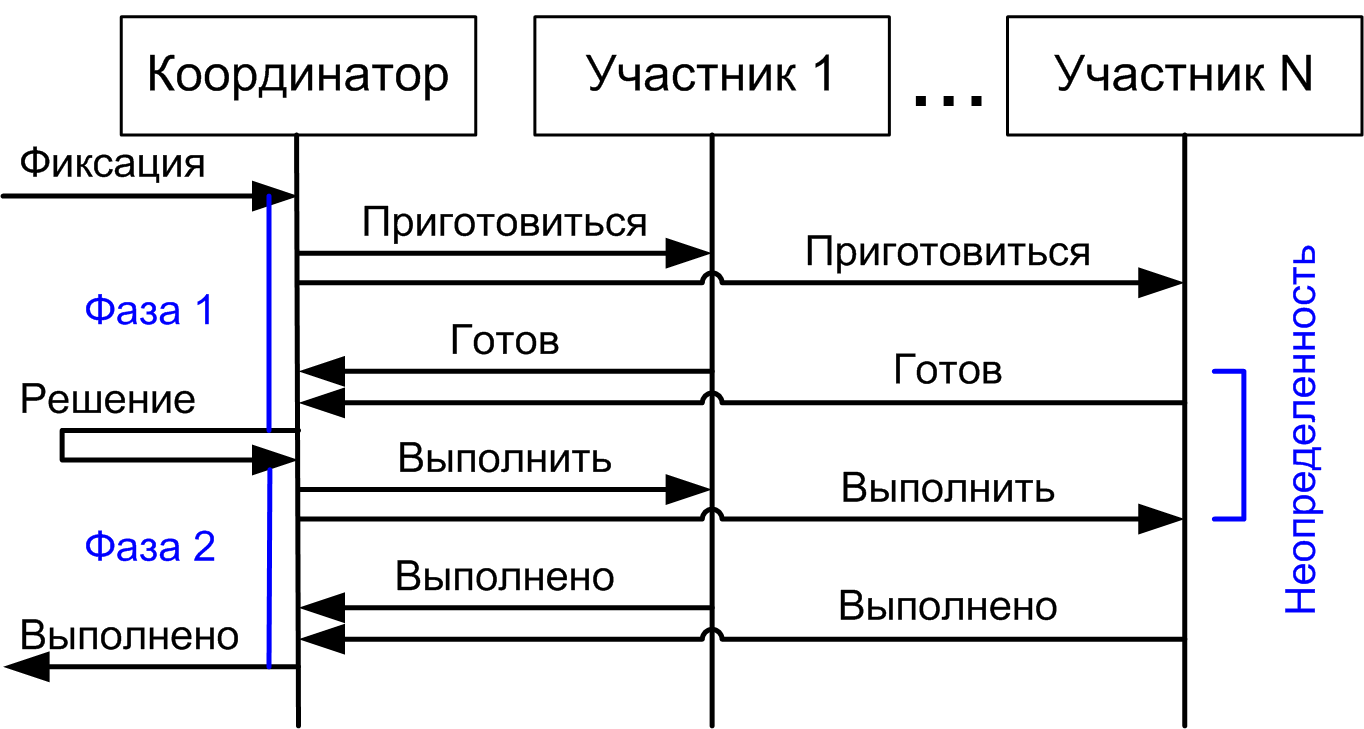
\includegraphics[width=0.8\textwidth]{../assets/kgeorgiy/distributed/Distributed_TwoPhase.png}
	\caption{Схема протокола двухфазной транзакции}
	\label{2-phase-tx}
\end{figure}

\begin{itemize}
	\item \textbf{Фаза подготовки}. Координатор рассылает информацию об изменении всем другим
	      копиям. Далее эти копии должны ответить, что готовы зафиксировать изменение (нет противоречий,
	      данные находятся в согласованном состоянии, нет иных ошибок).
	\item \textbf{Решение координатора}. После получения ответов от всех копий, координатор
	      принимает решение, выполнять ли фиксацию данных. Решение положительное, если от все пришедшие
	      ответы от других копий положительные.
	\item \textbf{Фаза выполнения}. При положительном решении координатор рассылает сообщение о
	      том, что изменения должны быть зафиксированы, и ожидает подтверждения этого от всех копий.
	\item \textbf{Результат}. Если координатор получает подтверждения от всех копий, то транзакция
	      считается выполненной.
\end{itemize}

Если \textit{координатор} не получил хотя бы одно подтверждение на первой фазе, то транзакция
автоматически откатывается. Как только принимается решение о фиксации, оно записывается в журнал
транзакций координатора -- так копии смогут заново воспроизвести решение при восстановлении.
Однако, если координатор не получил хотя бы одно подтверждение на второй фазе, то это неразрешимая
ситуация.

\textit{Копии} при сбое до отправки подтверждения на первой фазе должны откатить
транзакцию, поскольку координатор не мог принять решения о фиксации без подтверждения. При сбое до
получения решения о фиксации копия должна запросить решение снова у координатора. При получении
решения о фиксации копия записывает в свой журнал транзакций изменение для восстановления в
будущем.

Однако, задача теоретически не разрешима. То есть существует сценарий, при котором ни координатор,
ни реплика не смогут продвинуться (но эти случаи вырождены). Это показывает отсутствие решения
следующей задачи.

\paragraph{Задача двух генералов}

Генералам двух армий необходимо напасть на врага. Они достигнут успеха только если нападут
одновременно. Им необходимо прийти к \textit{консенсусу}: нападать или нет. Генералы могут
посылать гонцов с сообщениями, которых могут убить в пути.

\begin{proposition}
	Не существует гарантированного решения задачи двух генералов.
\end{proposition}

\begin{proof}
	Предположим противное: существует конечный протокол, при использовании которого можно прийти к
	консенсусу. Следовательно, существует минимальное по включению множество сообщений, которые
	необходимо отправить. Предположим, что последнее сообщение не было доставлено. Тогда невозможно
	принять решение. Противоречие.
\end{proof}

\paragraph{Протоколы предполагаемой фиксации и отката}

Как было показано выше, копии могут запрашивать решение у координатора повторно. Таким образом,
координатору необходимо сохранить информацию о решении до тех пор, пока не получит подтверждения от
всех копий. Рассмотрим два подхода оптимизации объема памяти, занимаемого решениями координатора.

\begin{itemize}
	\item \textbf{Протокол предполагаемой фиксации}. При решении о фиксации транзакции она
	      ``забывается'' координатором. Если координатор получает запрос о решении по неизвестной ему
	      транзакции, то он отвечает, что ее нужно зафиксировать. Данный подход позволяет сэкономить память,
	      если число зафиксированных транзакций сильно превышает число откаченных.
	\item \textbf{Протокол предполагаемого отката}. При решении об откате транзакции она
	      ``забывается'' координатором. Если координатор получает запрос о решении по неизвестной ему
	      транзакции, то он отвечает, что ее нужно откатить. Данный подход позволяет сэкономить память, если
	      число откаченных транзакций сильно превышает число зафиксированных.
\end{itemize}

\begin{remark}
	Протокол предполагаемой фиксации может привести к ложной фиксации. Например, если информация о
	решении была ошибочно утеряна. В таком случае всем другим участникам будет приходить ответ о
	фиксации, которой в действительности не было. Поэтому рекомендуется использовать протокол
	предполагаемого отката.
\end{remark}
